\documentclass{exam}
\usepackage{tikz}
\usepackage{amssymb}
\usepackage{amsmath}
\title{CS113/DISCRETE MATHEMATICS-SPRING 2024}
\author{Worksheet 22}
\date{Topic: Graph Terminology and Special Types of Graphs}
\begin{document}
\maketitle
\vspace{5mm}
\begin{center}
\fbox{\fbox{\parbox{5.5in}{\centering Today, we'll dive into the intriguing world of graphs and explore some special types, with a major focus on bipartite graphs. Happy Learning!}}}
\end{center}
\vspace{5mm}

\makebox[0.75\textwidth]{Student's Name and ID:\enspace\hrulefill} 

\vspace{5mm}
\makebox[0.75\textwidth]{Instructor’s name:\enspace\hrulefill}

\vspace{5mm}

\section{Bipartite Graphs:}
A simple graph $G$ is called bipartite if its vertex set $V$ can be partitioned into two disjoint sets $V_1$ and $V_2$ such that every edge in the graph connects a vertex in $V_1$ and a vertex in $V_2$ (so that no edge in $G$ connects either two vertices in $V_1$ or two vertices in $V_2$). When this condition holds, we call the pair $(V_1, V_2)$ a bipartition of the vertex set $V$ of $G$.

The following Theorem provides a useful criterion for determining whether a graph is bipartite.

\section{Theorem:}
A simple graph is bipartite if and only if it is possible to assign one of two different colors to
each vertex of the graph so that no two adjacent vertices are assigned the same color.

\vspace{5mm}

\begin{questions}

\question
Describe a graph model that represents whether each person at a party knows the name of each other person at the
party. Should the edges be directed or undirected? Should
multiple edges be allowed? Should loops be allowed?
\vspace{9in}

\question 
Can a simple graph exist with 15 vertices each of degree
five?
\newpage 

\question
. Show that in a simple graph with at least two vertices
there must be two vertices that have the same degree.
\newpage

\question
Determine whether the graph is bipartite.
You may find it useful to apply Theorem and answer the
question by determining whether it is possible to assign either red or blue to each vertex so that no two adjacent vertices are assigned the same color.

\begin{parts}
\part
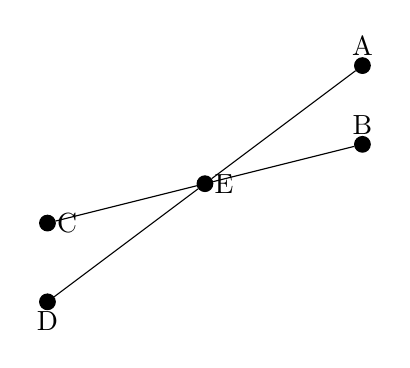
\begin{tikzpicture}
\node[circle, draw, fill, inner sep=2 pt] (A) at (6,1.5) {};
\node[circle, draw, fill, inner sep=2pt] (B) at (6,0.5) {};
\node[circle, draw, fill, inner sep=2pt] (C) at (2,-0.5) {};
\node[circle, draw, fill, inner sep=2pt] (D) at (2,-1.5) {};
\node[circle, draw, fill, inner sep=2pt] (E) at (4,0) {};

\node[above] at (A) {A};
\node[above] at (B) {B};
\node[right] at (C) {C};
\node[below] at (D) {D};
\node[right] at (E) {E};

\draw (A) -- (E);
\draw (B) -- (E);
\draw (C) -- (E);
\draw (D) -- (E);
\end{tikzpicture}
\vspace{3in}

\part
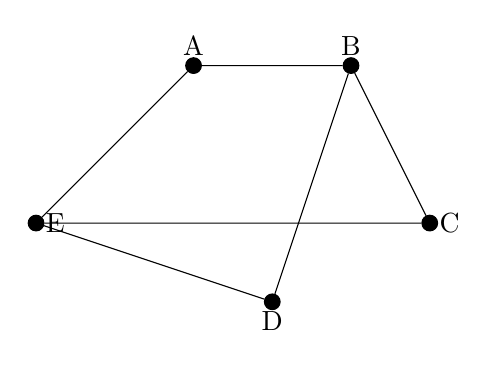
\begin{tikzpicture}
\node[circle, draw, fill, inner sep=2pt] (A) at (0,2) {};
\node[circle, draw, fill, inner sep=2pt] (B) at (2,2) {};
\node[circle, draw, fill, inner sep=2pt] (C) at (3,0) {};
\node[circle, draw, fill, inner sep=2pt] (D) at (1,-1) {};
\node[circle, draw, fill, inner sep=2pt] (E) at (-2,0) {};

\node[above] at (A) {A};
\node[above] at (B) {B};
\node[right] at (C) {C};
\node[below] at (D) {D};
\node[right] at (E) {E};

\draw (A) -- (B) -- (C) -- (E);
\draw (A)--(E);
\draw (D) -- (B);
\draw (E) -- (D);
\end{tikzpicture}
\vspace{3in}

\part
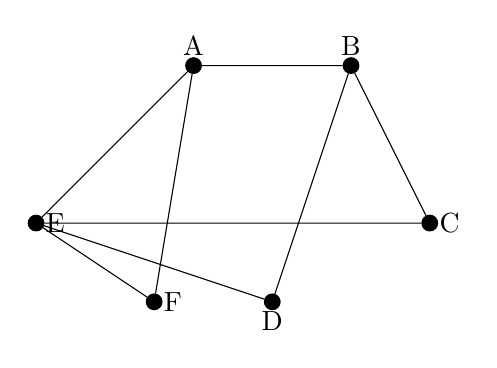
\begin{tikzpicture}
\node[circle, draw, fill, inner sep=2pt] (A) at (0,2) {};
\node[circle, draw, fill, inner sep=2pt] (B) at (2,2) {};
\node[circle, draw, fill, inner sep=2pt] (C) at (3,0) {};
\node[circle, draw, fill, inner sep=2pt] (D) at (1,-1) {};
\node[circle, draw, fill, inner sep=2pt] (E) at (-2,0) {};
\node[circle, draw, fill, inner sep=2pt] (F) at (-0.5,-1) {};

\node[above] at (A) {A};
\node[above] at (B) {B};
\node[right] at (C) {C};
\node[below] at (D) {D};
\node[right] at (E) {E};
\node[right] at (F) {F};
\draw (A) -- (B) -- (C) -- (E);
\draw (A)--(E);
\draw (D) -- (B);
\draw (E) -- (D);
\draw (A) -- (F);
\draw (E) -- (F);
\end{tikzpicture}
\vspace{3in}

\part
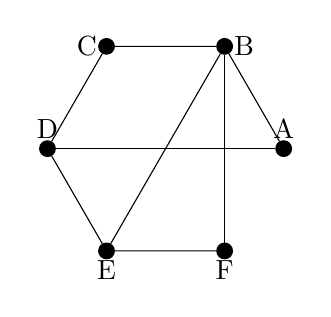
\begin{tikzpicture}
\foreach \i/\letter in {0/A, 60/B, 120/C, 180/D, 240/E, 300/F}
\node[circle, draw, fill, inner sep=2pt] (\letter) at (\i:1.5) {};
\node[above] at (A) {A};
\node[right] at (B) {B};
\node[left] at (C) {C};
\node[above] at (D) {D};
\node[below] at (E) {E};
\node[below] at (F) {F};


\draw (A) -- (B) -- (C) -- (D) -- (E) -- (F);
\draw (B)--(F);
\draw (B)--(E);
\draw (A)--(D);


\end{tikzpicture}

\end{parts}




\end{questions}
\end{document}

